
\section{Разработка архитектуры наземной станции}
Аппаратная часть наземной станции состоит из:

--- компьютера,

--- передающего модуля радиоуправления,

--- видеоприемника,

--- устройства приема-передачи телеметрии

К компьютеру по UART порту подключается модуль радиоуправления. Через USB порт подключается видеоприемник. Устройство приема-передачи телеметрии также подключается к компьютеру по UART порту. Настраиваем видеоприемник на частоту, соответствующую частоте видеопередатчика квадрокоптера и приступаем к настройке программной части.

Программная часть представляет собой совокупность взаимодействущего программного обеспечения, включающего в себя:

--- операционную систему на базе ядра linux,
--- qgroundcontrol,

--- web-браузер,

--- консоль

В qgroundcontrol выставляется бод-рейт. 115200 -- максимально доступный для используемого. Далее происходит подключение и обмен данными с устройством приема-передачи телеметрии, расположенного на борту квадрокоптера.
По MAVLink протоколу передаются данные в указанный UART, и все программы, прослушивающие этот UART порт имеют доступ к данным с борта квадрокоптера. Для взаимодействия через ROS инструменты необходима настройка всех параметров подключения. На данном этапе НИР используется готовой решение от Copter Express -- пакет clover, позволяющий производить настройку максимально просто. В launch файлах пакета прописываются все параметры. Указываем UART, бауд-рейт, и в консоли запускаем clover с помощью команд:
\begin{MyCode}
gs@groundstation:~$ source /home/clover/catkin\_ws/devel/setup.bash
gs@groundstation:~$ roslaunch clover clover.launch
\end{MyCode}

После этого доступны все инструменты ROS. На листинге \ref{lst:1} приведен результат выполнения команды для получения телеметрии. "frame\_id: ''" означает, что показания берутся в системе координат относительно квадрокоптера.
\begin{Program}[H]
	\caption{Вывод телеметрии квадрокоптера в консоли} \label{lst:1}
	\begin{MyCode}
gs@groundstation:~$ rosservice call /get_telemetry "frame_id: ''" 
frame_id: "map"
connected: True
armed: False
mode: "MANUAL"
x: -0.00260298536159
y: -6.72723326716e-05
z: 0.00103790743742
lat: 0.0
lon: 0.0
alt: 0.0
vx: -0.00717502878979
vy: -0.00176917202771
vz: 0.00364218326285
pitch: 0.0221049506217
roll: -0.0172985047102
yaw: 0.000302107335301
pitch_rate: 0.00245076417923
roll_rate: 0.00449034944177
yaw_rate: 0.00266480189748
voltage: 12.1499996185
cell_voltage: 4.05000019073
gs@groundstation:~$
	\end{MyCode}
\end{Program}

Видеоприемник подключен в устройствах как /dev/video0. Указываем его в launch-файле, перезагружаем clover и проверяем в web-браузере топики по адресу localhost:8080 (рис. \ref{fig:topic}).

\begin{figure}[H]
	\centering
	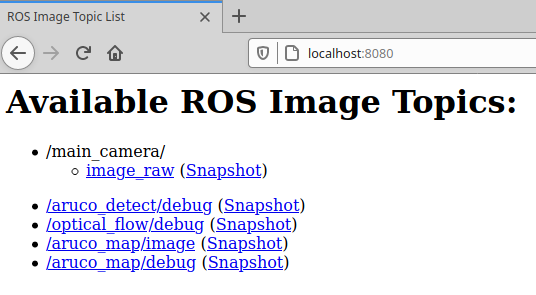
\includegraphics[width=0.5\linewidth]{pics/topic}
	\caption{Список топиков, доступный по умолчанию
	}
	\label{fig:topic}
\end{figure}

Список топиков также меняется в launch файлах. В image raw топике будет отображаться видеопоток, полученный видеоприемником с борта квадрокоптера, в остальных топиках публикуются:

--- aruco-detect (на image raw определяются с помощью openCV aruco маркеры),

--- optical flow (на изображение с image raw накладывается точка отсчета для лазерного дальномера),

--- aruco map (карта маркеров, прописанная в конфигурационном файле).

Aruco маркеры -- маркеры, напоминающие QR коды, созданные для позиционирования робототехнических систем с использованием компьютерного зрения.

Aruco-detect -- НОДа ROS для распознавания карты маркеров. На ее основе планируется реализация системы навигации и позиционирования квадрокоптера для наземной станции. 

